\subsection{Entity-Relationship Schema}

We decided to develop our project using as stepping stone the database designed by the e-team group during the FTB course. The original database's ER schema can be seen in Figure \ref{er_original}, while the relational schema is presented in Figure \ref{ls_original}.
\\
\newgeometry{top=0.1cm, bottom=0.1cm}
\begin{figure}[H]
\centering
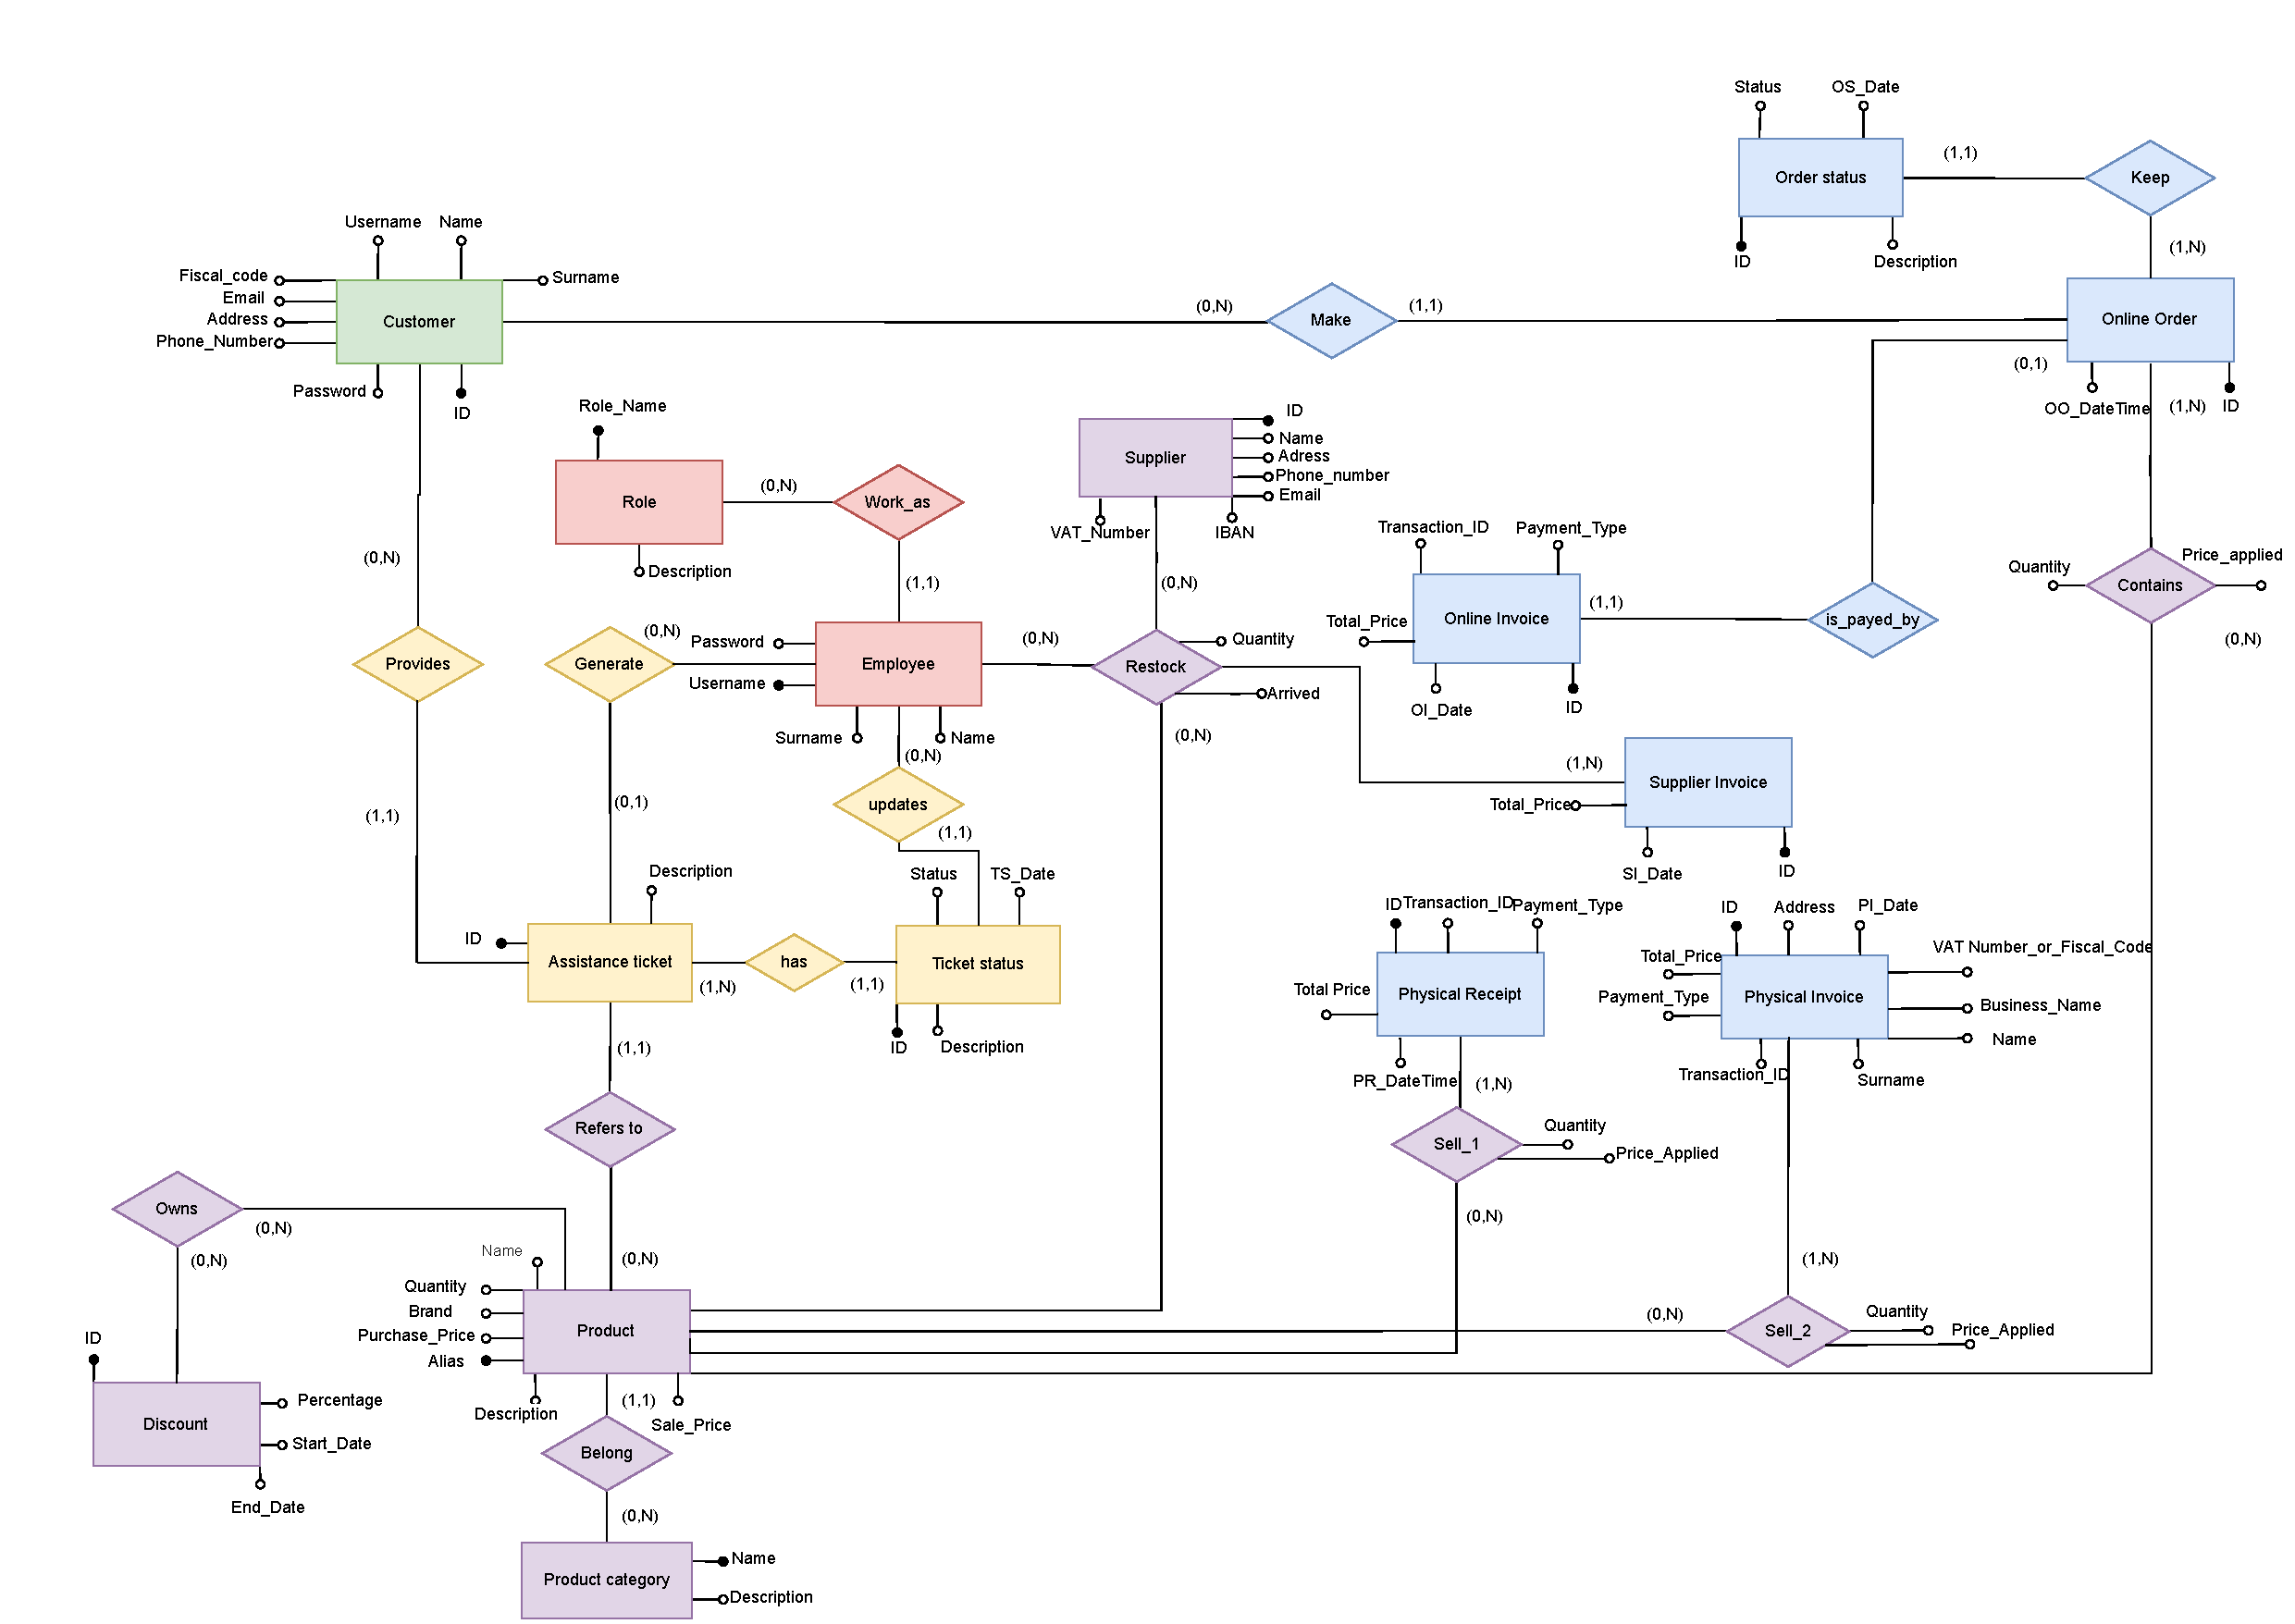
\includegraphics[width=\textwidth]{Schemas/ER_original.drawio.pdf}
\caption{Original ER schema designed by e-team}
\label{er_original}
\end{figure}

\begin{figure}[H]
\centering
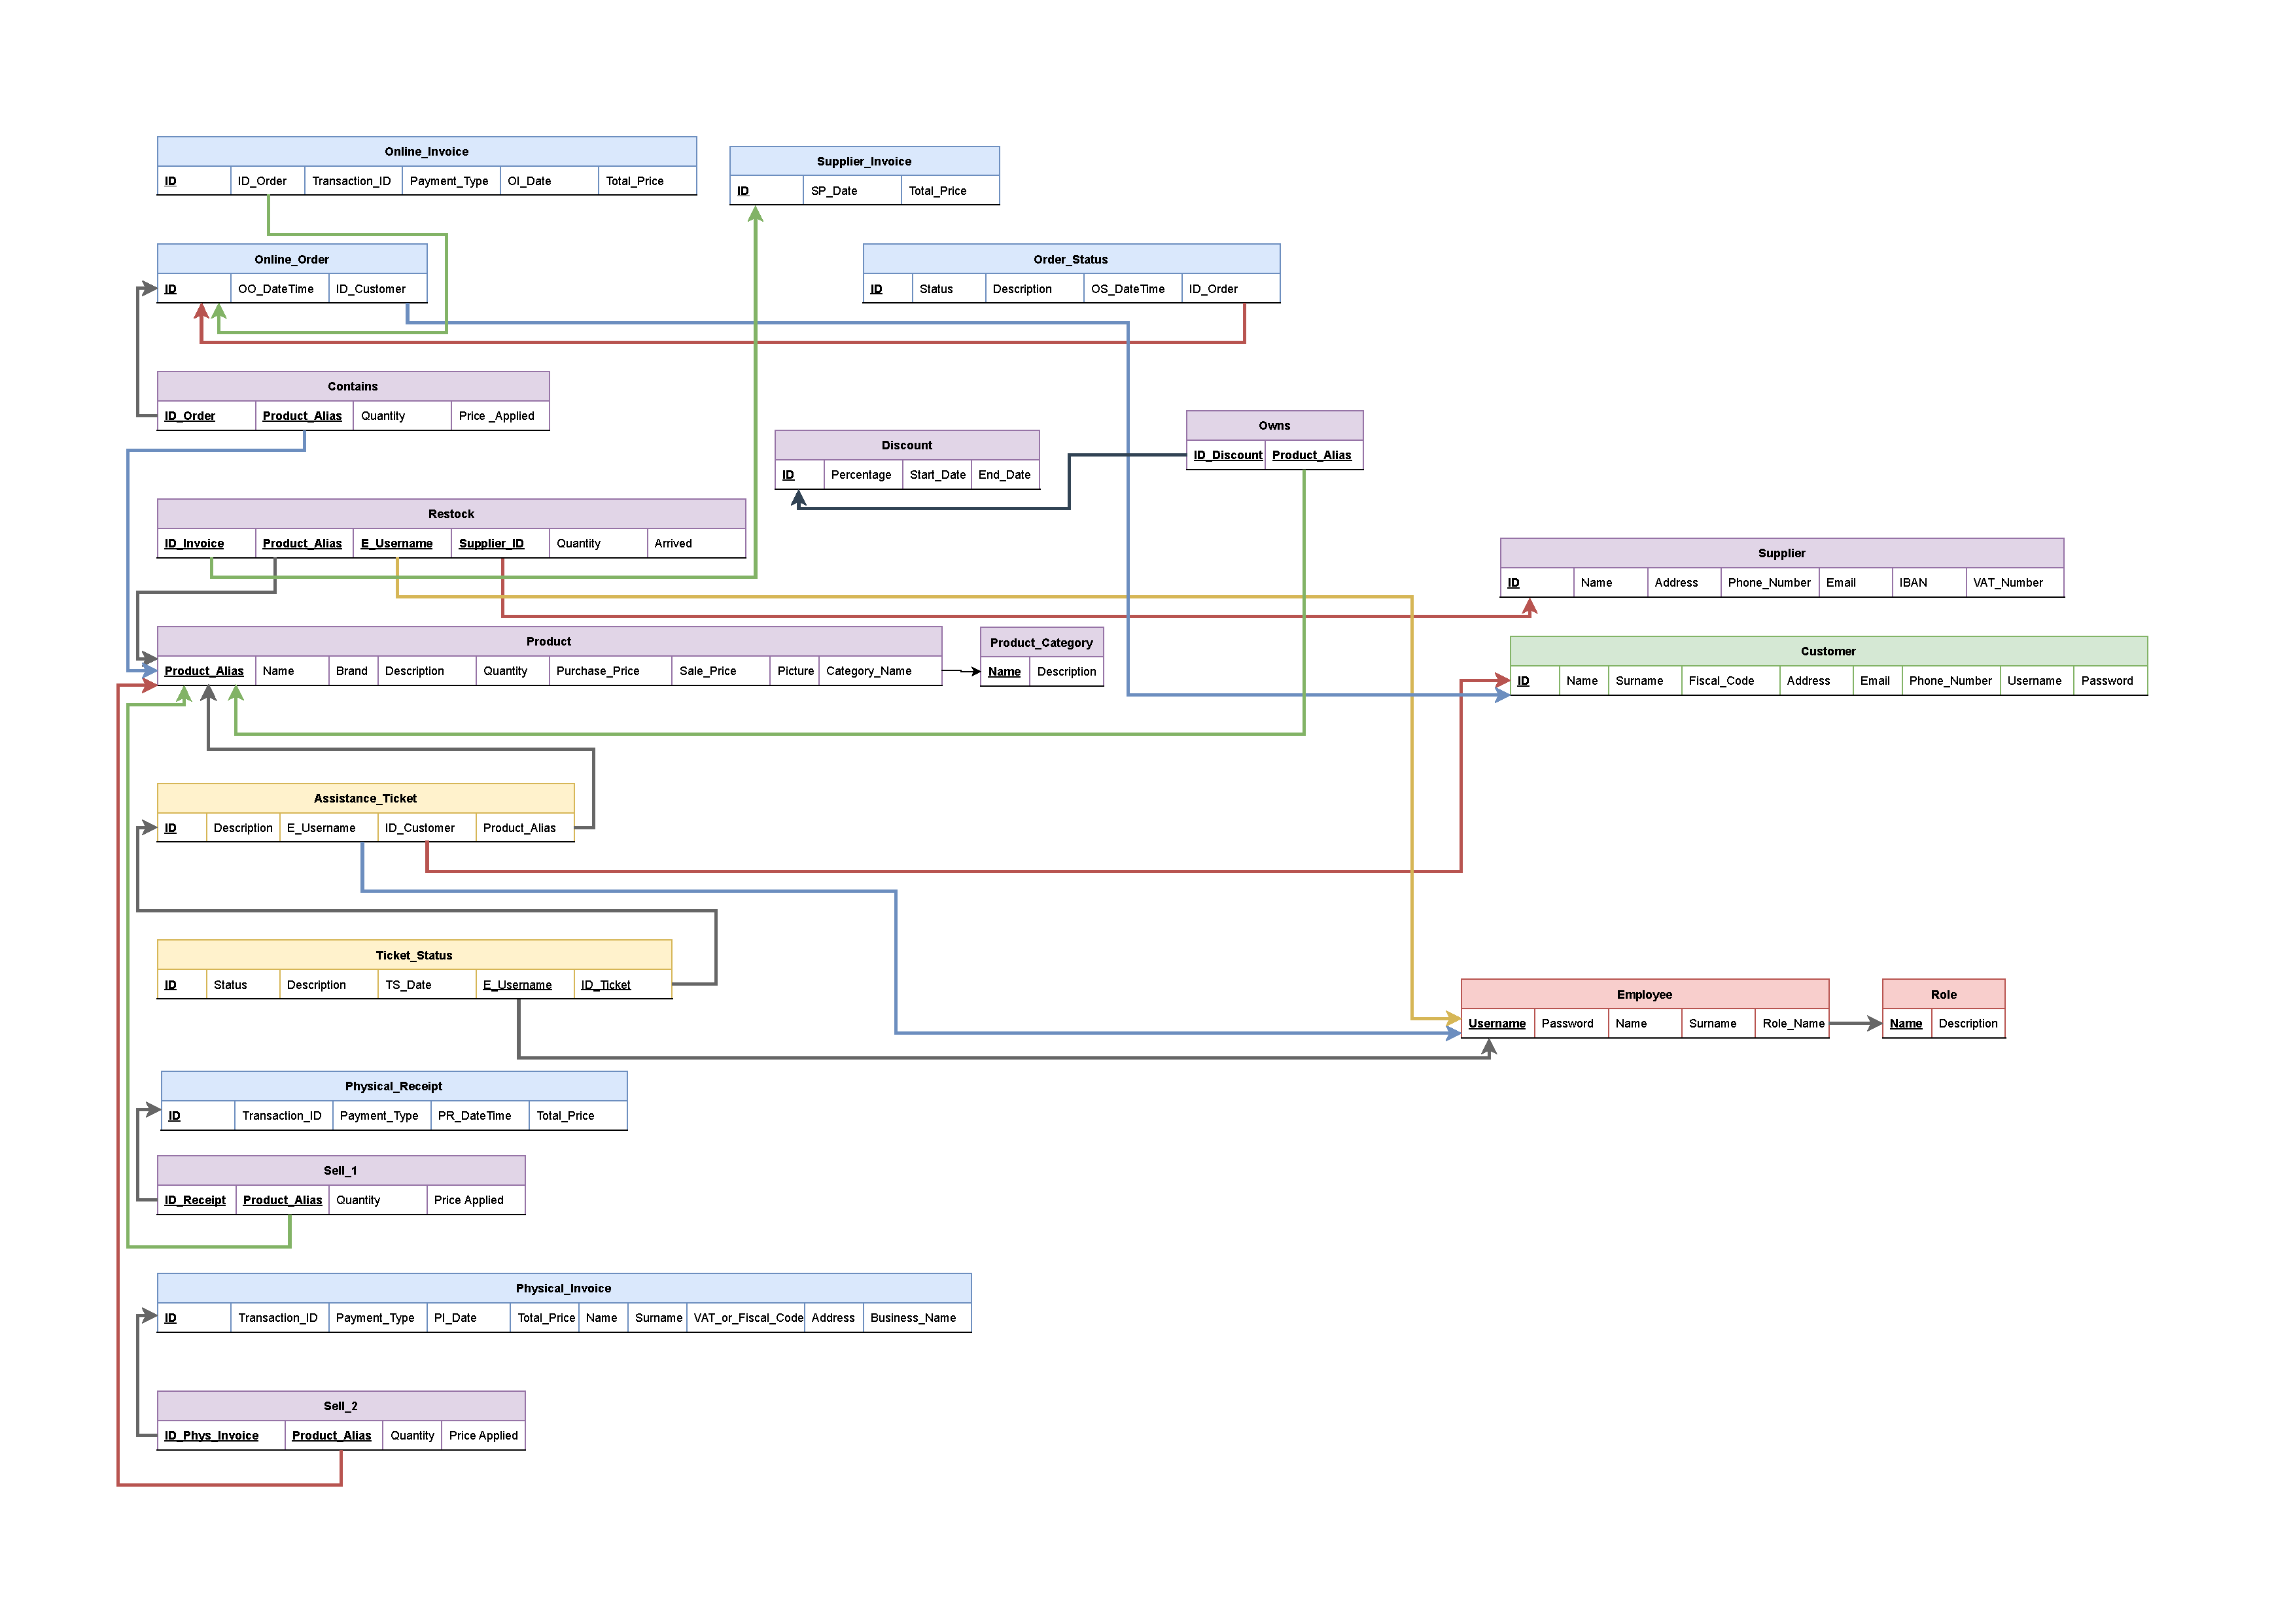
\includegraphics[width=\textwidth]{Schemas/LogicRS_original.drawio.pdf}
\caption{Original Relational schema designed by e-team}
\label{ls_original}
\end{figure}
\restoregeometry
In order to maintain the project manageable, we decided to cut some relations. In particular, we decided to remove all the "offline services" and to build our web application only to manage the online side of the shop.
We also removed the management of the supplier, dedicating the development of our project only to the services seen by the client of the shop (excluding the management of the employees that is needed in our web application since we needed them to setting up the permission). In Figure \ref{er_modified} and \ref{ls_modified} are reported the final version of the design for the data layer (ER schema and relational schema respectively).

\begin{figure}[H]
\centering
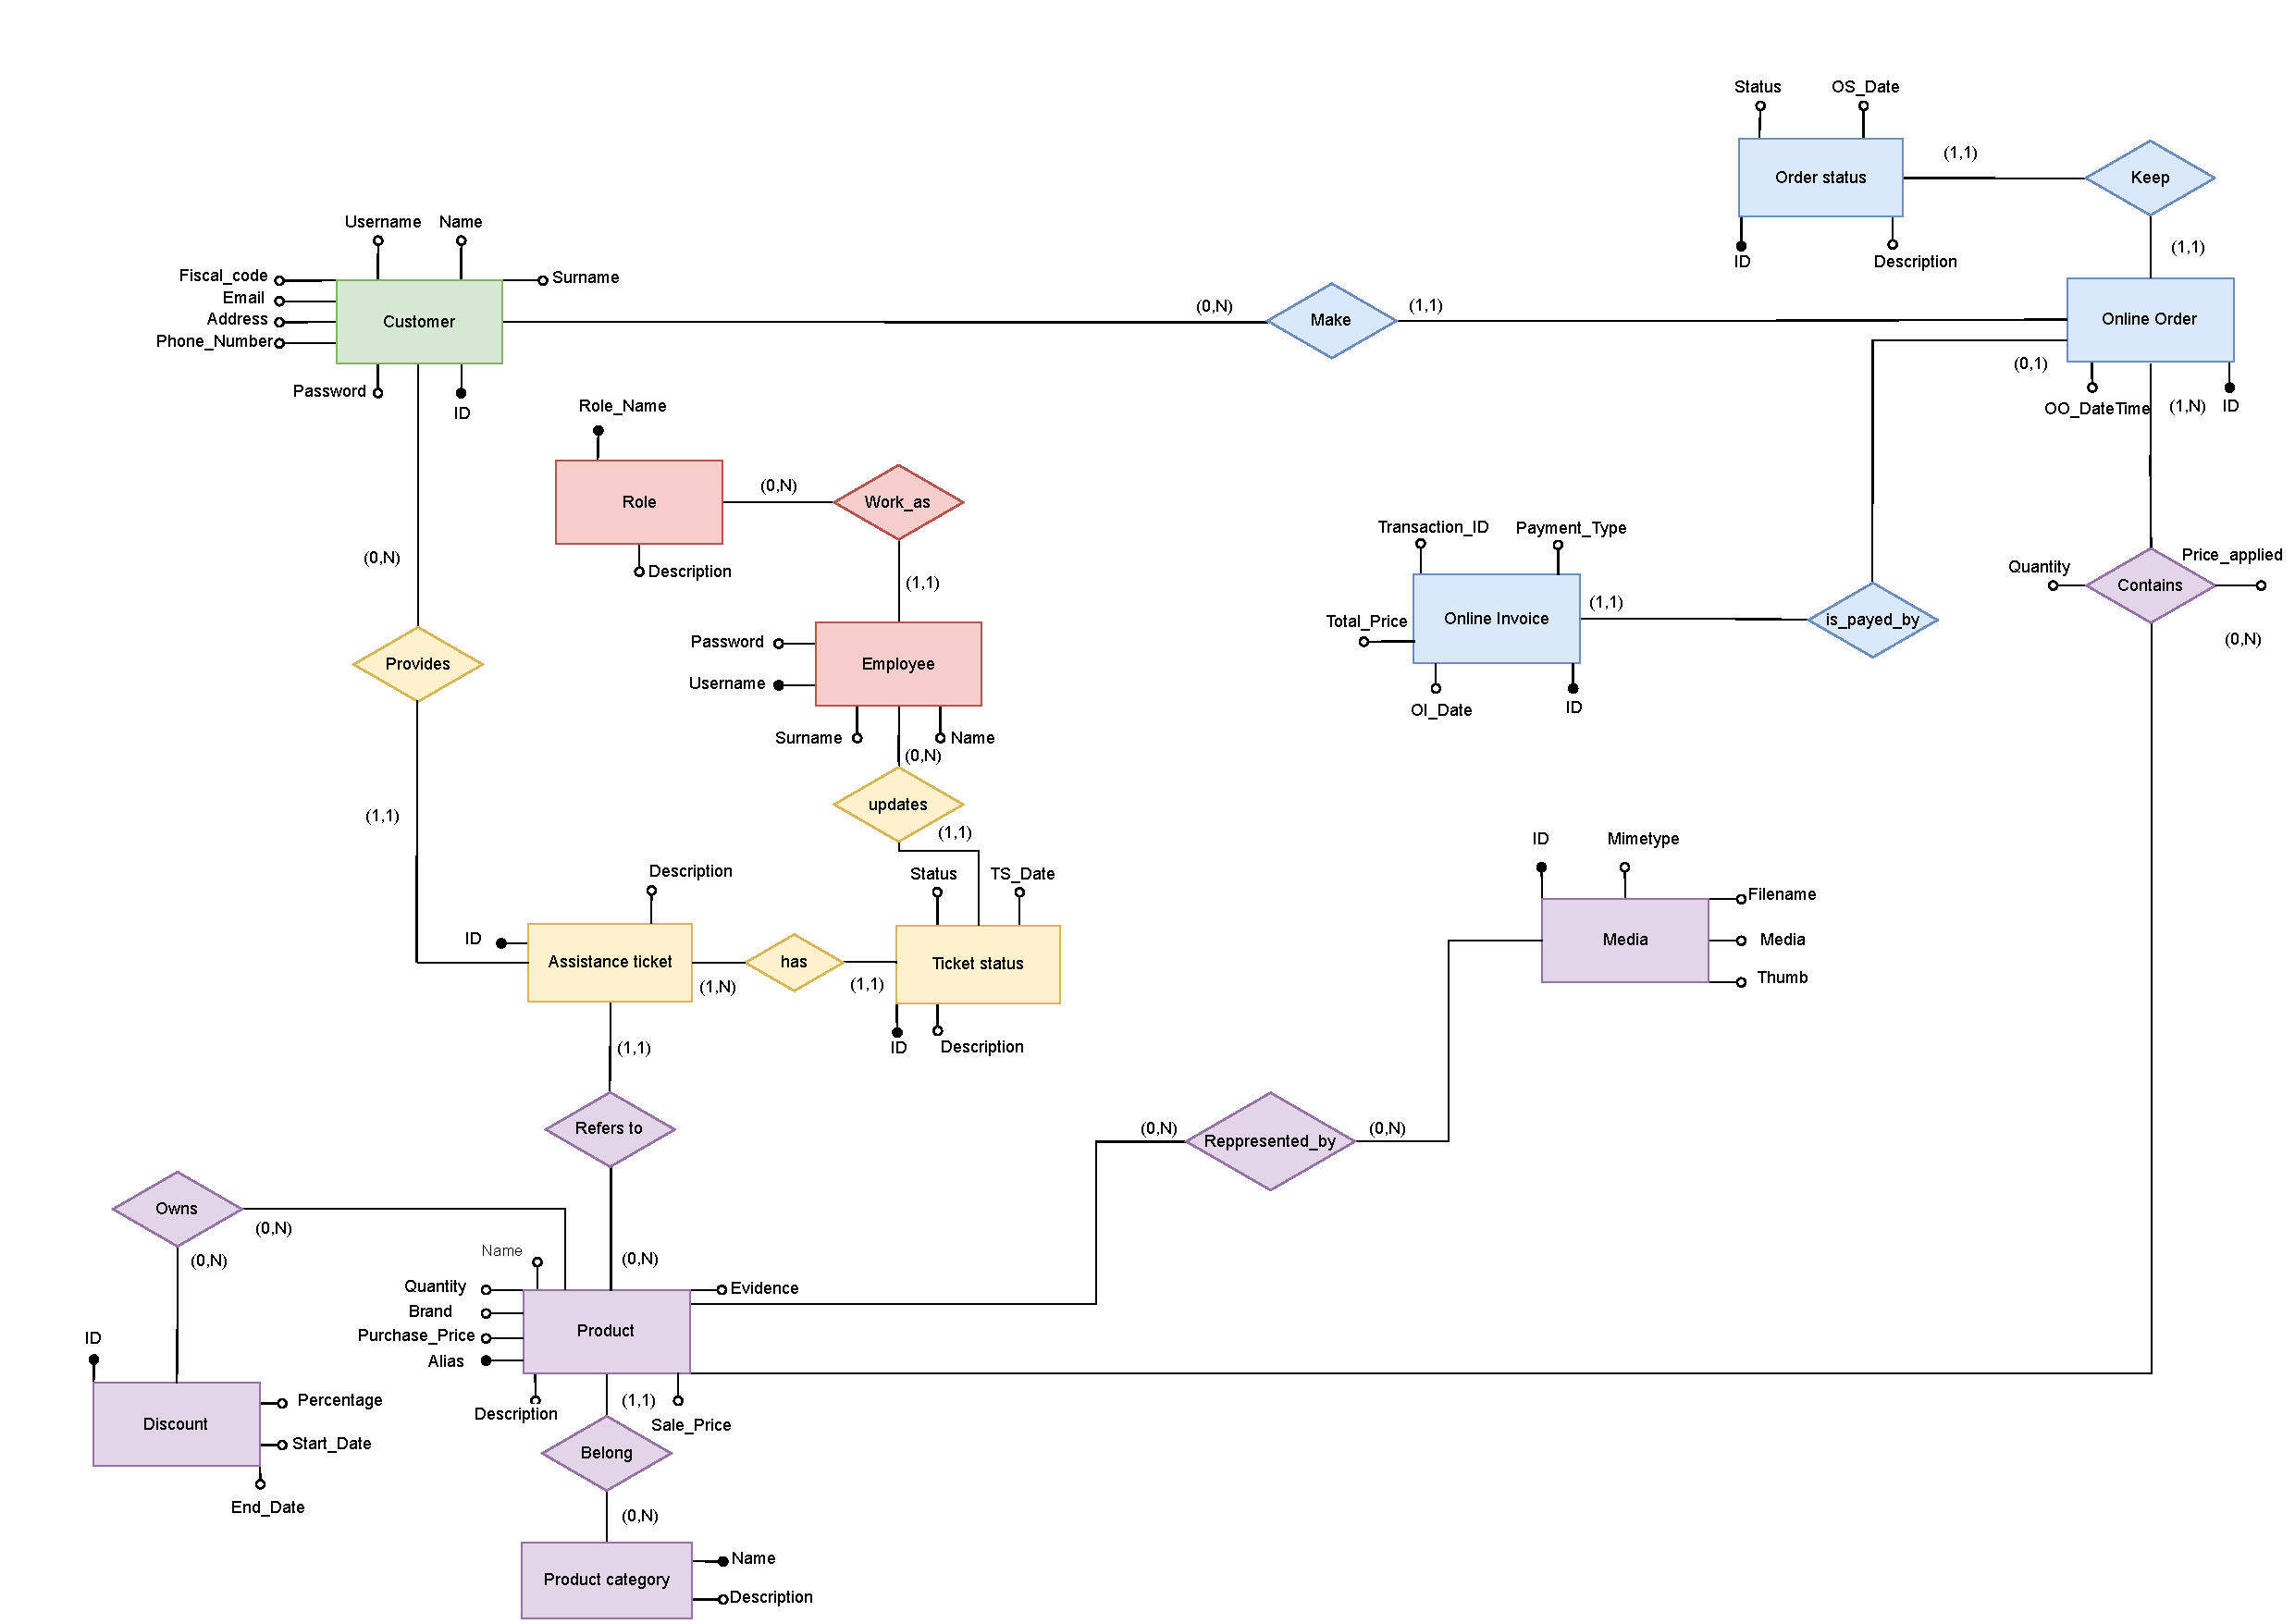
\includegraphics[width=\textwidth]{Schemas/ER_modified.drawio.pdf}
\caption{ER schema modified}
\label{er_modified}
\end{figure}

\begin{figure}[H]
\centering
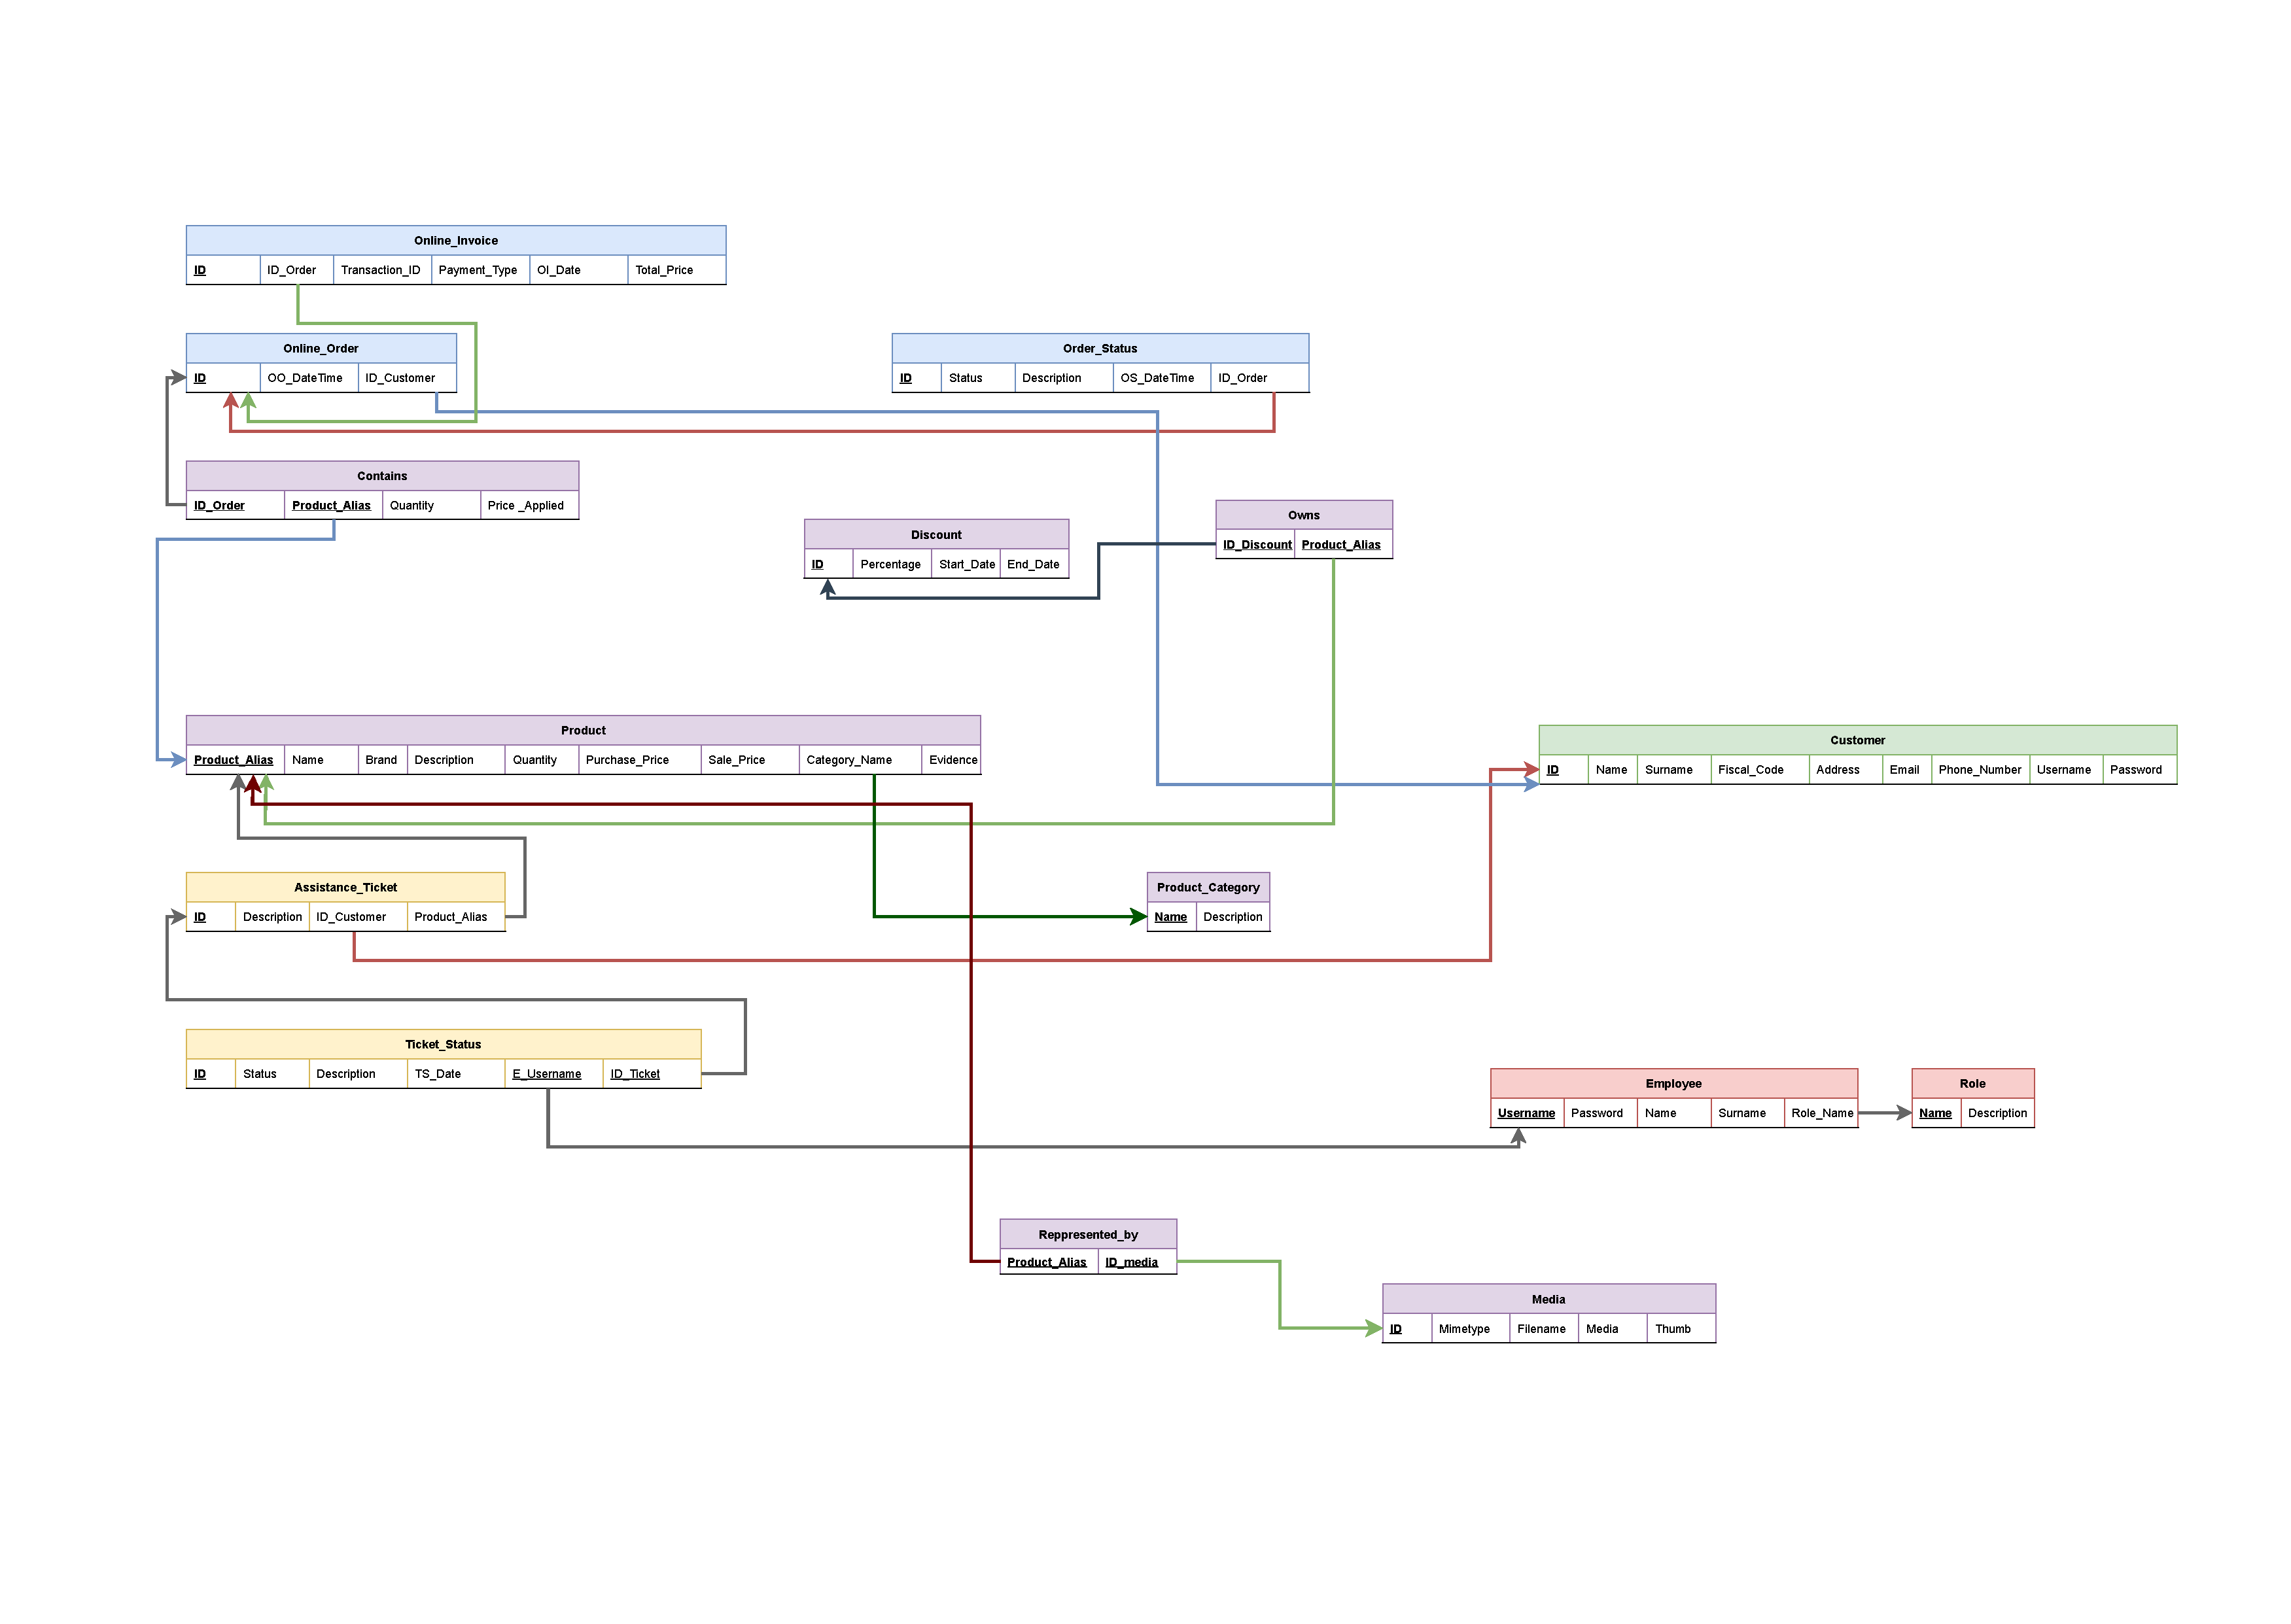
\includegraphics[width=\textwidth]{Schemas/LogicRS_modified.drawio.pdf}
\caption{Relational schema modified}
\label{ls_modified}
\end{figure}